%!TEX program = xelatex
\PassOptionsToPackage{table,svgnames}{xcolor}
\PassOptionsToPackage{english}{translator}
\documentclass[aspectratio=169,11pt]{beamer}

%----------------------------------------
% Packages
%----------------------------------------
%\usepackage[utf8]{inputenc}
\usepackage[T1]{fontenc}
\usepackage[english]{babel} % Second language = main language
\usepackage{translator}
\usepackage{lmodern}
\usepackage{hyperref}
\usepackage{xcolor}
\usepackage{listings}
\usepackage{amsmath}
\usepackage{amssymb}
\usepackage{mathrsfs}
\usepackage{array}
\usepackage{tabularx}
\usepackage{multirow}
\usepackage[justification=centering]{caption}
\usepackage{float}
\usepackage{standalone}
\usepackage{import}
% PGF-TikZ
\usepackage{pgf}
\usepackage{tikz}
\usepackage{pgf-umlsd}
\usepackage{pgfgantt}

%----------------------------------------
% Theme
%----------------------------------------

% \usetheme{boxes}
% \useoutertheme{infolines}
% \usecolortheme{whale}%beaver
% \usecolortheme{seagull}

\usetheme[illustration=cover]{utbm}
%\usetheme{utbm}

% remove bottom line
%\setbeamertemplate{footline}{}

% remove navigation symbols.
\beamertemplatenavigationsymbolsempty{}

%\setbeamercovered{transparent}

%----------------------------------------
% Informations
%----------------------------------------

\title{Generation of the hyperplanes of  \texorpdfstring{$S_k(3)$}{S\_k(3)} }
\subtitle{TX52}
\author{Jérôme Boulmier, Maxime Pinard}
\institute[UTBM]{Université de Technologie de Belfort Montbéliard}
\date[2018-06-29]{29 June 2018}

%\keywords{}
\subject{TX52, Generation of the geometric hyperplanes of  \texorpdfstring{$S_k(3)$}{S\_k(3)}}
%\logo{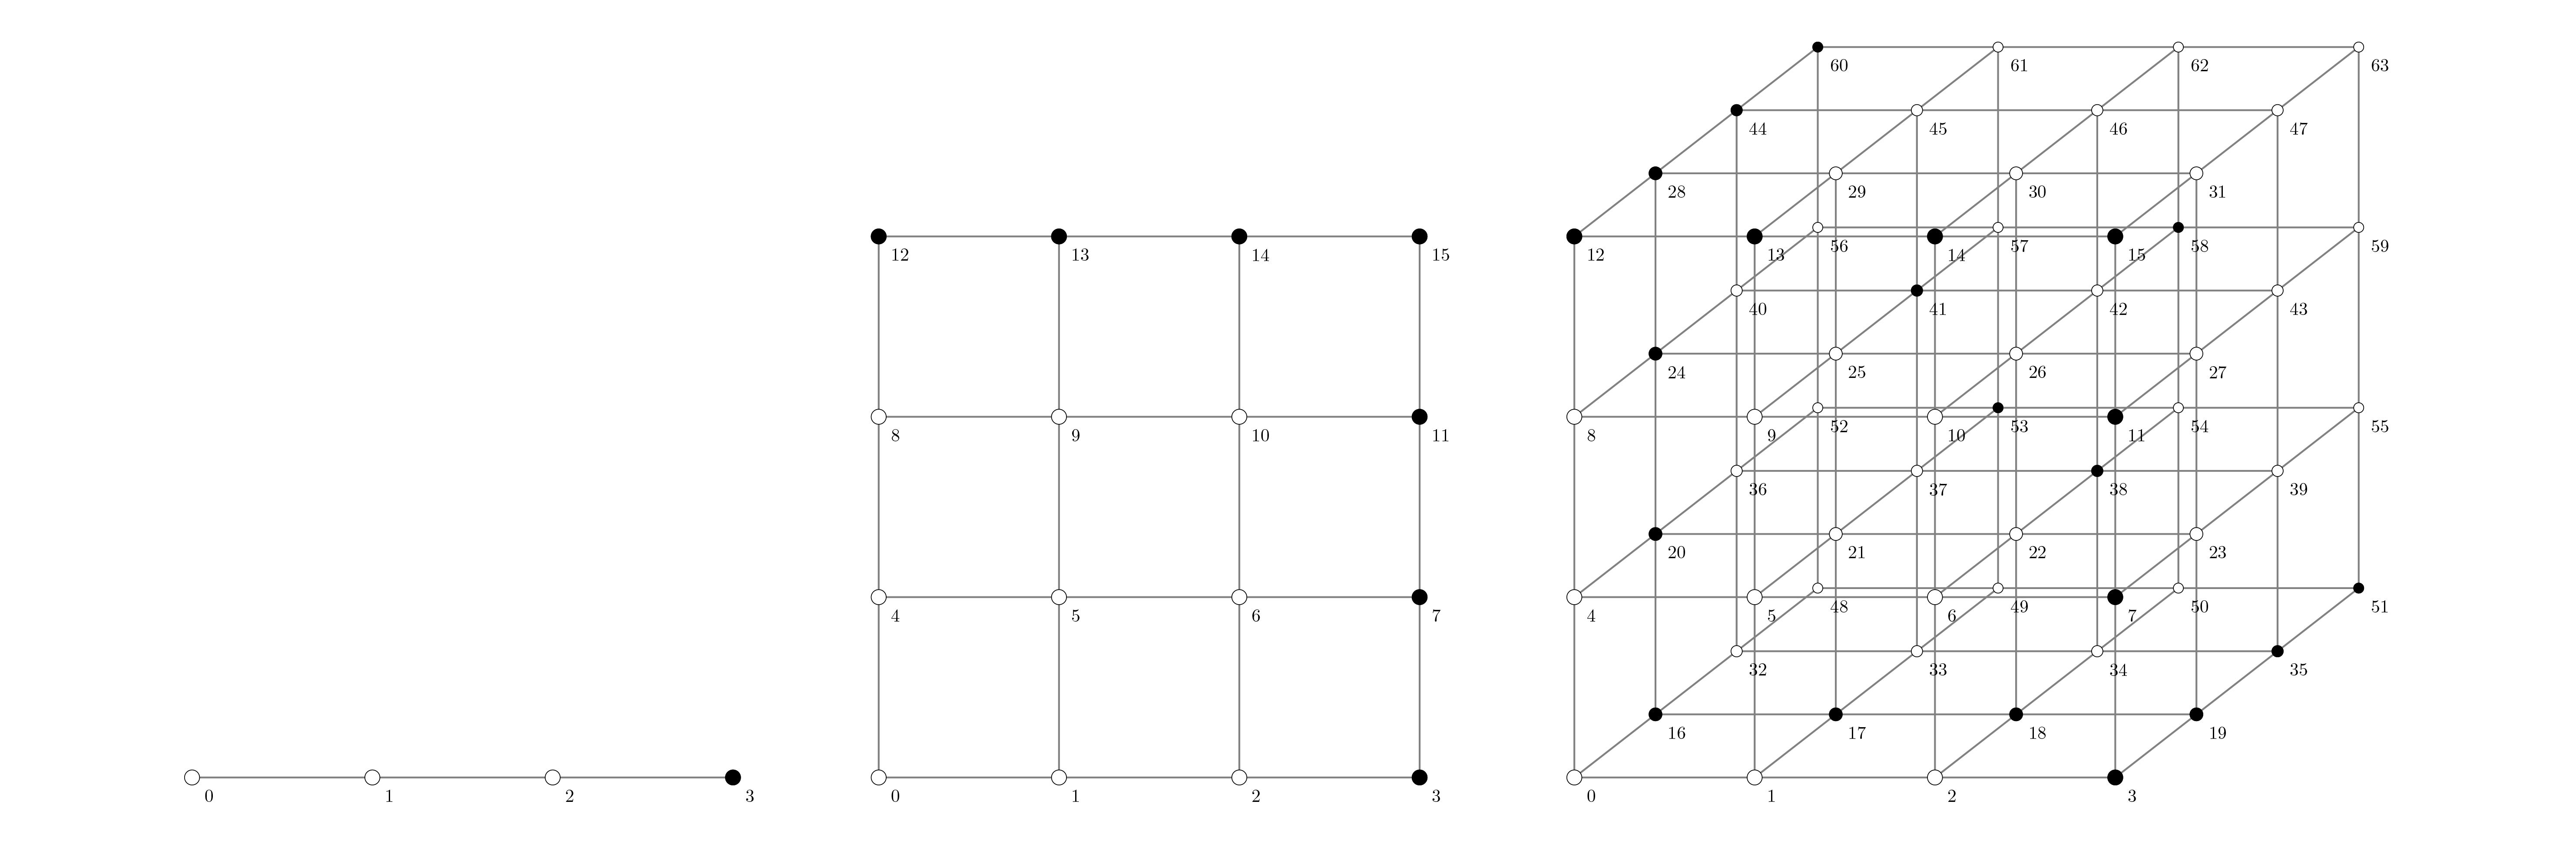
\includegraphics[width=0.12\textwidth]{cover}}

%----------------------------------------
% Configurations
%----------------------------------------

\graphicspath{{figures/}}

% \AtBeginSection
% {
% 	\begin{frame}<beamer>
% 		\vfill{}
% 		\centering
% 		\begin{beamercolorbox}[sep=8pt,center]{title}
% 			\Huge\insertsectionhead\par%
% 		\end{beamercolorbox}
% 		\vfill{}
% 	\end{frame}
% }

\AtBeginSection
{
	\begin{frame}[plain]
		\utbmtitle{\insertsectionhead}
	\end{frame}
}

\makeatletter
\let\@@magyar@captionfix\relax
\makeatother

%----------------------------------------
% Figures configuration
%----------------------------------------

\usetikzlibrary{shapes.geometric}
\usetikzlibrary{arrows.meta}
\usetikzlibrary{calc}
\usetikzlibrary{matrix}
\usetikzlibrary{fit}


%---------------------------------
% Colors
\colorlet{points_boder_color}{black}%
\colorlet{points_color}{white}%
\colorlet{in_points_color}{black}%
\colorlet{lines_color}{gray}%

%---------------------------------
% Sizes
\pgfmathsetmacro\pointssep{100}%
\pgfmathsetmacro\pointssize{10}%
\pgfmathsetmacro\lineswidth{1}%

\newcommand{\inPoints}{}

%----------------------------------------
% Document
%----------------------------------------
\begin{document}
	\begin{frame}[plain,noframenumbering]
		\titlepage
	\end{frame}
	\begin{frame}{Table of contents}
		\tableofcontents
	\end{frame}
	\section{Working space: \texorpdfstring{$S_k(3)$}{S\_k(3)}}
		%!TEX root = ./main.tex

\begin{frame}
	%---------------------------------
	% Geometry
	\pgfmathsetmacro\dimension{2}% in [0,3]
	\pgfmathsetmacro\pointsPerLine{3}% in [1,\infty[

	%---------------------------------
	% Auto config
	\pgfmathsetmacro\xdim{\dimension>0}%
	\pgfmathsetmacro\ydim{\dimension>1}%
	\pgfmathsetmacro\zdim{\dimension>2}%
	\pgfmathsetmacro\pointsPerLineMinusOne{\pointsPerLine-1}%
	\pgfmathsetmacro\xnbr{\pointsPerLineMinusOne*\xdim}%
	\pgfmathsetmacro\ynbr{\pointsPerLineMinusOne*\ydim}%
	\pgfmathsetmacro\znbr{\pointsPerLineMinusOne*\zdim}%

	\resizebox{\textwidth}{!}{
		\begin{tikzpicture}[x={(1pt,0pt)},y={(0pt,1pt)},z={(0.45pt,0.35pt)},>=Latex]
			\tikzset{point/.style={
				draw,
				circle,
				minimum size=\pointsize,
				inner sep=0,
			}}

			% Coordinates
			\foreach \x in {0,...,\xnbr}
			{
				\foreach \y in {0,...,\ynbr}
				{
					\foreach \z in {0,...,\znbr}
					{
						\pgfmathsetmacro\num{int(\x+(\pointsPerLine*\y)+(\pointsPerLine*\pointsPerLine*\z))}
						\coordinate (point\num) at (\pointssep*\x,\pointssep*\y,\pointssep*\z) {};
						\coordinate (point_\x_\y_\z) at (\pointssep*\x,\pointssep*\y,\pointssep*\z) {};
					}
				}
			}

			% Lines
			\foreach \x in {0,...,\xnbr}
			{
				\foreach \y in {0,...,\ynbr}
				{
					\foreach \z in {0,...,\znbr}
					{
						\ifthenelse{\x=0}{}{
							\pgfmathsetmacro\lastx{int(\x-1)}
							\draw[line width=\lineswidth,lines_color] (point_\lastx_\y_\z) -- (point_\x_\y_\z);
						}
						\ifthenelse{\y=0}{}{
							\pgfmathsetmacro\lasty{int(\y-1)}
							\draw[line width=\lineswidth,lines_color] (point_\x_\lasty_\z) -- (point_\x_\y_\z);
						}
						\ifthenelse{\z=0}{}{
							\pgfmathsetmacro\lastz{int(\z-1)}
							\draw[line width=\lineswidth,lines_color] (point_\x_\y_\lastz) -- (point_\x_\y_\z);
						}
					}
				}
			}

			% Points and numbers
			\foreach \x in {0,...,\xnbr}
			{
				\foreach \y in {0,...,\ynbr}
				{
					\foreach \z in {0,...,\znbr}
					{
						% Config
						\pgfmathsetmacro\num{int(\x+(\pointsPerLine*\y)+(\pointsPerLine*\pointsPerLine*\z))}
						\pgfmathsetmacro\pointsize{\pointssize*5/(5+\z+1)}

						% Draw point
						\node[
							point,
							points_boder_color,
							fill=points_color
						] at (point_\x_\y_\z.center) {};

						% Number
						\pgfmathsetmacro\num{int(\x+(\pointsPerLine*\y)+(\pointsPerLine*\pointsPerLine*\z))}
						\uncover<1>{
							\node[below right=3pt] at (point_\x_\y_\z.center) {(\x, \y)};
						}
						\uncover<2->{
							\node[below right=3pt] at (point_\x_\y_\z.center) {$\x e_0 + \y e_1$};
						}
					}
				}
			}

			\uncover<1>{
				\draw[->,thick,blue] (point_0_0_0.center) -- node[above] {x} (point_1_0_0.center);
				\draw[->,thick,blue] (point_0_0_0.center) -- node[right] {y} (point_0_1_0.center);
			}
			\uncover<2>{
				\draw[->,thick,blue] (point_0_0_0.center) -- node[above] {$e_0$} (point_1_0_0.center);
				\draw[->,thick,blue] (point_0_0_0.center) -- node[right] {$e_1$} (point_0_1_0.center);
			}
			\uncover<3->{
				\draw[->,thick,red] (point_0_0_0.center) -- node[above right] {$e_0$} (point_2_0_0.center);
				\draw[->,thick,green] (point_0_0_0.center) -- node[above right] {$e_1$} (point_0_2_0.center);
				\draw[->,thick,blue] (point_0_0_0.center) -- node[above left] {$e_0 + e_1$} (point_2_2_0.center);
				\draw[->,thick,purple] (point_0_0_0.center) to[out=22.5,in=-90] node[below right] {$2 e_0 + e_1$} (point_2_1_0.center) to[out=90,in=0] (point_1_2_0.center);
			}

			\node[anchor=center] at (3.5*\pointssep, \pointssep) {
				\begin{minipage}{120pt}
					\centering%
					$GF(3) \otimes GF(3)$\\
					\uncover<2->{
						$\alpha e_0 + \beta e_1,\ (\alpha, \beta) \in \mathbb{F}_3$\\
					}
					\hfil\\
					\uncover<3->{
						4 directions:
						\begin{itemize}
							\item $e_0$
							\item $e_1$
							\item $e_0 + e_1$
							\item $2 e_0 + e_1$
						\end{itemize}
						\hfil\\
						\hfil\\
						$P(GF(3) \times GF(3))$\\
					}
					\uncover<4->{
						$=$\\
						$PG(1,3)$\\
					}
				\end{minipage}
			};

			\node at (4.5*\pointssep, \pointssep) {};
		\end{tikzpicture}
	}%
	\begin{tikzpicture}[remember picture,overlay,x={(1pt,0pt)},y={(0pt,1pt)}]
		\node[anchor=south east] at ($(current page.south east)+(-3,10)$) {\tiny\textit{$GF(3) = \mathbb{F}_3$, GF stands for Gallois Field}};
	\end{tikzpicture}
\end{frame}

		%!TEX root = ./main.tex

\begin{frame}
	%---------------------------------
	% Geometry
	\pgfmathsetmacro\dimension{1}% in [0,3]
	\pgfmathsetmacro\pointsPerLine{4}% in [1,\infty[

	%---------------------------------
	% Auto config
	\pgfmathsetmacro\xdim{\dimension>0}%
	\pgfmathsetmacro\ydim{\dimension>1}%
	\pgfmathsetmacro\zdim{\dimension>2}%
	\pgfmathsetmacro\pointsPerLineMinusOne{\pointsPerLine-1}%
	\pgfmathsetmacro\xnbr{\pointsPerLineMinusOne*\xdim}%
	\pgfmathsetmacro\ynbr{\pointsPerLineMinusOne*\ydim}%
	\pgfmathsetmacro\znbr{\pointsPerLineMinusOne*\zdim}%

	\resizebox{\textwidth}{!}{
		\begin{tikzpicture}[x={(1pt,0pt)},y={(0pt,1pt)},z={(0.45pt,0.35pt)},>=Latex]
			\tikzset{point/.style={
				draw,
				circle,
				minimum size=\pointsize,
				inner sep=0,
			}}

			% Coordinates
			\foreach \x in {0,...,\xnbr}
			{
				\foreach \y in {0,...,\ynbr}
				{
					\foreach \z in {0,...,\znbr}
					{
						\pgfmathsetmacro\num{int(\x+(\pointsPerLine*\y)+(\pointsPerLine*\pointsPerLine*\z))}
						\coordinate (point\num) at (\pointssep*\x,\pointssep*\y,\pointssep*\z) {};
						\coordinate (point_\x_\y_\z) at (\pointssep*\x,\pointssep*\y,\pointssep*\z) {};
					}
				}
			}

			% Lines
			\foreach \x in {0,...,\xnbr}
			{
				\foreach \y in {0,...,\ynbr}
				{
					\foreach \z in {0,...,\znbr}
					{
						\ifthenelse{\x=0}{}{
							\pgfmathsetmacro\lastx{int(\x-1)}
							\draw[line width=\lineswidth,lines_color] (point_\lastx_\y_\z) -- (point_\x_\y_\z);
						}
						\ifthenelse{\y=0}{}{
							\pgfmathsetmacro\lasty{int(\y-1)}
							\draw[line width=\lineswidth,lines_color] (point_\x_\lasty_\z) -- (point_\x_\y_\z);
						}
						\ifthenelse{\z=0}{}{
							\pgfmathsetmacro\lastz{int(\z-1)}
							\draw[line width=\lineswidth,lines_color] (point_\x_\y_\lastz) -- (point_\x_\y_\z);
						}
					}
				}
			}

			% Points and numbers
			\foreach \x in {0,...,\xnbr}
			{
				\foreach \y in {0,...,\ynbr}
				{
					\foreach \z in {0,...,\znbr}
					{
						% Config
						\pgfmathsetmacro\num{int(\x+(\pointsPerLine*\y)+(\pointsPerLine*\pointsPerLine*\z))}
						\pgfmathsetmacro\pointsize{\pointssize*5/(5+\z+1)}

						% Draw point
						\node[
							point,
							points_boder_color,
							fill=points_color
						] at (point_\x_\y_\z.center) {};
					}
				}
			}

			\uncover<1>{
				\node[below right=3pt] at (point_0_0_0.center) {$e_0$};
				\node[below right=3pt] at (point_1_0_0.center) {$e_1$};
				\node[below right=3pt] at (point_2_0_0.center) {$e_0 + e_1$};
				\node[below right=3pt] at (point_3_0_0.center) {$2 e_0 + e_1$};
			}
			\uncover<2->{
				\node[below right=3pt] at (point_0_0_0.center) {0};
				\node[below right=3pt] at (point_1_0_0.center) {1};
				\node[below right=3pt] at (point_2_0_0.center) {2};
				\node[below right=3pt] at (point_3_0_0.center) {3};
			}

			\node[anchor=center] at (4.5*\pointssep, 0) {
				\begin{minipage}{120pt}
					\centering%
					$PG(1,3)$
				\end{minipage}
			};

			\node at (5.5*\pointssep, 0) {};
		\end{tikzpicture}
	}%
	\begin{tikzpicture}[remember picture,overlay,x={(1pt,0pt)},y={(0pt,1pt)}]
		\node[anchor=south east] at ($(current page.south east)+(-3,10)$) {\tiny\textit{PG stands for Projective Geometry}};
	\end{tikzpicture}
\end{frame}

		%!TEX root = ./main.tex

\pgfmathsetmacro\pointsPerLine{4}% in [1,\infty[
\newsavebox\geometrya
\sbox{\geometrya}{%
	\pgfmathsetmacro\dimension{1}% in [0,3]
	%---------------------------------
% Auto config
\pgfmathsetmacro\xdim{\dimension>0}%
\pgfmathsetmacro\ydim{\dimension>1}%
\pgfmathsetmacro\zdim{\dimension>2}%
\pgfmathsetmacro\pointsPerLineMinusOne{\pointsPerLine-1}%
\pgfmathsetmacro\xnbr{\pointsPerLineMinusOne*\xdim}%
\pgfmathsetmacro\ynbr{\pointsPerLineMinusOne*\ydim}%
\pgfmathsetmacro\znbr{\pointsPerLineMinusOne*\zdim}%

%---------------------------------
% Figure
\begin{tikzpicture}[x={(1pt,0pt)},y={(0pt,1pt)},z={(0.45pt,0.35pt)}]
	\tikzset{point/.style={
		draw,
		circle,
		minimum size=\pointsize,
		inner sep=0,
	}}

	% Coordinates
	\foreach \x in {0,...,\xnbr}
	{
		\foreach \y in {0,...,\ynbr}
		{
			\foreach \z in {0,...,\znbr}
			{
				\pgfmathsetmacro\num{int(\x+(\pointsPerLine*\y)+(\pointsPerLine*\pointsPerLine*\z))}
				\coordinate (point\num) at (\pointssep*\x,\pointssep*\y,\pointssep*\z) {};
				\coordinate (point_\x_\y_\z) at (\pointssep*\x,\pointssep*\y,\pointssep*\z) {};
			}
		}
	}

	% Lines
	\foreach \x in {0,...,\xnbr}
	{
		\foreach \y in {0,...,\ynbr}
		{
			\foreach \z in {0,...,\znbr}
			{
				\ifthenelse{\x=0}{}{
					\pgfmathsetmacro\lastx{int(\x-1)}
					\draw[line width=\lineswidth,lines_color] (point_\lastx_\y_\z) -- (point_\x_\y_\z);
				}
				\ifthenelse{\y=0}{}{
					\pgfmathsetmacro\lasty{int(\y-1)}
					\draw[line width=\lineswidth,lines_color] (point_\x_\lasty_\z) -- (point_\x_\y_\z);
				}
				\ifthenelse{\z=0}{}{
					\pgfmathsetmacro\lastz{int(\z-1)}
					\draw[line width=\lineswidth,lines_color] (point_\x_\y_\lastz) -- (point_\x_\y_\z);
				}
			}
		}
	}

	% Points and numbers
	\foreach \x in {0,...,\xnbr}
	{
		\foreach \y in {0,...,\ynbr}
		{
			\foreach \z in {0,...,\znbr}
			{
				% Config
				\pgfmathsetmacro\num{int(\x+(\pointsPerLine*\y)+(\pointsPerLine*\pointsPerLine*\z))}
				\pgfmathsetmacro\pointsize{\pointssize*5/(5+\z+1)}

				% Draw point
				\node[
					point,
					points_boder_color,
					fill=points_color
				] at (point_\x_\y_\z.center) {};

				% Fill point if is in
				\foreach \i in \inPoints
				{
					\ifthenelse{\num=\i}{
						\node[
							point,
							points_boder_color,
							fill=in_points_color
						] at (point\i.center) {};
					}{}
				}

				% Number
				\pgfmathsetmacro\num{int(\x+(\pointsPerLine*\y)+(\pointsPerLine*\pointsPerLine*\z))}
				\node[below right=3pt] at (point_\x_\y_\z.center) {\small\num};
			}
		}
	}
\end{tikzpicture}
%
}
\newsavebox\geometryb
\sbox{\geometryb}{%
	\pgfmathsetmacro\dimension{2}% in [0,3]
	%---------------------------------
% Auto config
\pgfmathsetmacro\xdim{\dimension>0}%
\pgfmathsetmacro\ydim{\dimension>1}%
\pgfmathsetmacro\zdim{\dimension>2}%
\pgfmathsetmacro\pointsPerLineMinusOne{\pointsPerLine-1}%
\pgfmathsetmacro\xnbr{\pointsPerLineMinusOne*\xdim}%
\pgfmathsetmacro\ynbr{\pointsPerLineMinusOne*\ydim}%
\pgfmathsetmacro\znbr{\pointsPerLineMinusOne*\zdim}%

%---------------------------------
% Figure
\begin{tikzpicture}[x={(1pt,0pt)},y={(0pt,1pt)},z={(0.45pt,0.35pt)}]
	\tikzset{point/.style={
		draw,
		circle,
		minimum size=\pointsize,
		inner sep=0,
	}}

	% Coordinates
	\foreach \x in {0,...,\xnbr}
	{
		\foreach \y in {0,...,\ynbr}
		{
			\foreach \z in {0,...,\znbr}
			{
				\pgfmathsetmacro\num{int(\x+(\pointsPerLine*\y)+(\pointsPerLine*\pointsPerLine*\z))}
				\coordinate (point\num) at (\pointssep*\x,\pointssep*\y,\pointssep*\z) {};
				\coordinate (point_\x_\y_\z) at (\pointssep*\x,\pointssep*\y,\pointssep*\z) {};
			}
		}
	}

	% Lines
	\foreach \x in {0,...,\xnbr}
	{
		\foreach \y in {0,...,\ynbr}
		{
			\foreach \z in {0,...,\znbr}
			{
				\ifthenelse{\x=0}{}{
					\pgfmathsetmacro\lastx{int(\x-1)}
					\draw[line width=\lineswidth,lines_color] (point_\lastx_\y_\z) -- (point_\x_\y_\z);
				}
				\ifthenelse{\y=0}{}{
					\pgfmathsetmacro\lasty{int(\y-1)}
					\draw[line width=\lineswidth,lines_color] (point_\x_\lasty_\z) -- (point_\x_\y_\z);
				}
				\ifthenelse{\z=0}{}{
					\pgfmathsetmacro\lastz{int(\z-1)}
					\draw[line width=\lineswidth,lines_color] (point_\x_\y_\lastz) -- (point_\x_\y_\z);
				}
			}
		}
	}

	% Points and numbers
	\foreach \x in {0,...,\xnbr}
	{
		\foreach \y in {0,...,\ynbr}
		{
			\foreach \z in {0,...,\znbr}
			{
				% Config
				\pgfmathsetmacro\num{int(\x+(\pointsPerLine*\y)+(\pointsPerLine*\pointsPerLine*\z))}
				\pgfmathsetmacro\pointsize{\pointssize*5/(5+\z+1)}

				% Draw point
				\node[
					point,
					points_boder_color,
					fill=points_color
				] at (point_\x_\y_\z.center) {};

				% Fill point if is in
				\foreach \i in \inPoints
				{
					\ifthenelse{\num=\i}{
						\node[
							point,
							points_boder_color,
							fill=in_points_color
						] at (point\i.center) {};
					}{}
				}

				% Number
				\pgfmathsetmacro\num{int(\x+(\pointsPerLine*\y)+(\pointsPerLine*\pointsPerLine*\z))}
				\node[below right=3pt] at (point_\x_\y_\z.center) {\small\num};
			}
		}
	}
\end{tikzpicture}
%
}
\newsavebox\geometryc
\sbox{\geometryc}{%
	\pgfmathsetmacro\dimension{3}% in [0,3]
	%---------------------------------
% Auto config
\pgfmathsetmacro\xdim{\dimension>0}%
\pgfmathsetmacro\ydim{\dimension>1}%
\pgfmathsetmacro\zdim{\dimension>2}%
\pgfmathsetmacro\pointsPerLineMinusOne{\pointsPerLine-1}%
\pgfmathsetmacro\xnbr{\pointsPerLineMinusOne*\xdim}%
\pgfmathsetmacro\ynbr{\pointsPerLineMinusOne*\ydim}%
\pgfmathsetmacro\znbr{\pointsPerLineMinusOne*\zdim}%

%---------------------------------
% Figure
\begin{tikzpicture}[x={(1pt,0pt)},y={(0pt,1pt)},z={(0.45pt,0.35pt)}]
	\tikzset{point/.style={
		draw,
		circle,
		minimum size=\pointsize,
		inner sep=0,
	}}

	% Coordinates
	\foreach \x in {0,...,\xnbr}
	{
		\foreach \y in {0,...,\ynbr}
		{
			\foreach \z in {0,...,\znbr}
			{
				\pgfmathsetmacro\num{int(\x+(\pointsPerLine*\y)+(\pointsPerLine*\pointsPerLine*\z))}
				\coordinate (point\num) at (\pointssep*\x,\pointssep*\y,\pointssep*\z) {};
				\coordinate (point_\x_\y_\z) at (\pointssep*\x,\pointssep*\y,\pointssep*\z) {};
			}
		}
	}

	% Lines
	\foreach \x in {0,...,\xnbr}
	{
		\foreach \y in {0,...,\ynbr}
		{
			\foreach \z in {0,...,\znbr}
			{
				\ifthenelse{\x=0}{}{
					\pgfmathsetmacro\lastx{int(\x-1)}
					\draw[line width=\lineswidth,lines_color] (point_\lastx_\y_\z) -- (point_\x_\y_\z);
				}
				\ifthenelse{\y=0}{}{
					\pgfmathsetmacro\lasty{int(\y-1)}
					\draw[line width=\lineswidth,lines_color] (point_\x_\lasty_\z) -- (point_\x_\y_\z);
				}
				\ifthenelse{\z=0}{}{
					\pgfmathsetmacro\lastz{int(\z-1)}
					\draw[line width=\lineswidth,lines_color] (point_\x_\y_\lastz) -- (point_\x_\y_\z);
				}
			}
		}
	}

	% Points and numbers
	\foreach \x in {0,...,\xnbr}
	{
		\foreach \y in {0,...,\ynbr}
		{
			\foreach \z in {0,...,\znbr}
			{
				% Config
				\pgfmathsetmacro\num{int(\x+(\pointsPerLine*\y)+(\pointsPerLine*\pointsPerLine*\z))}
				\pgfmathsetmacro\pointsize{\pointssize*5/(5+\z+1)}

				% Draw point
				\node[
					point,
					points_boder_color,
					fill=points_color
				] at (point_\x_\y_\z.center) {};

				% Fill point if is in
				\foreach \i in \inPoints
				{
					\ifthenelse{\num=\i}{
						\node[
							point,
							points_boder_color,
							fill=in_points_color
						] at (point\i.center) {};
					}{}
				}

				% Number
				\pgfmathsetmacro\num{int(\x+(\pointsPerLine*\y)+(\pointsPerLine*\pointsPerLine*\z))}
				\node[below right=3pt] at (point_\x_\y_\z.center) {\small\num};
			}
		}
	}
\end{tikzpicture}
%
}

\begin{frame}
	\begin{minipage}{\textwidth}
		\centering%
		$S_k(3) = \underbrace{PG(1,3) \otimes \dots \otimes PG(1,3)}_{k\text{ times}}$
	\end{minipage}
	\resizebox{\textwidth}{!}{
		\begin{tikzpicture}
			\uncover<2->{
				\node (geometrya) at (0,0) {\usebox{\geometrya}};
				\node[anchor=north,yshift=-15,font=\Huge] at (geometrya.south) {$S_1(3)$};
			}
			\uncover<3->{
				\node[anchor=south west, xshift=50] (geometryb) at (geometrya.south east) {\usebox{\geometryb}};
				\node[anchor=north,yshift=-15,font=\Huge] at (geometryb.south) {$S_2(3)$};
			}
			\uncover<4->{
				\node[anchor=south west, xshift=50] (geometryc) at (geometryb.south east) {\usebox{\geometryc}};
				\node[anchor=north,yshift=-15,font=\Huge] at (geometryc.south) {$S_3(3)$};
			}
		\end{tikzpicture}
	}
	\begin{tikzpicture}[remember picture,overlay,x={(1pt,0pt)},y={(0pt,1pt)}]
		\node[anchor=south east] at ($(current page.south east)+(-3,10)$) {\tiny\textit{S stands for Segre varieties}};
	\end{tikzpicture}
\end{frame}

	\begin{frame}[plain]
		\utbmclosingframe{Questions?}
	\end{frame}
\end{document}
